\documentclass[tikz,border=8pt]{standalone}
\usepackage[T1]{fontenc}
\usepackage{times}
\usetikzlibrary{positioning,arrows.meta,fit,backgrounds,calc,
                shapes.geometric,decorations.pathreplacing}
\definecolor{encC}{HTML}{4C72B0}
\definecolor{hypC}{HTML}{DD8452}
\definecolor{subsC}{HTML}{5A9E6F}
\definecolor{featC}{HTML}{7A6CB0}
\definecolor{fixC}{HTML}{B0544C}
\definecolor{darkC}{HTML}{343434}
\begin{document}
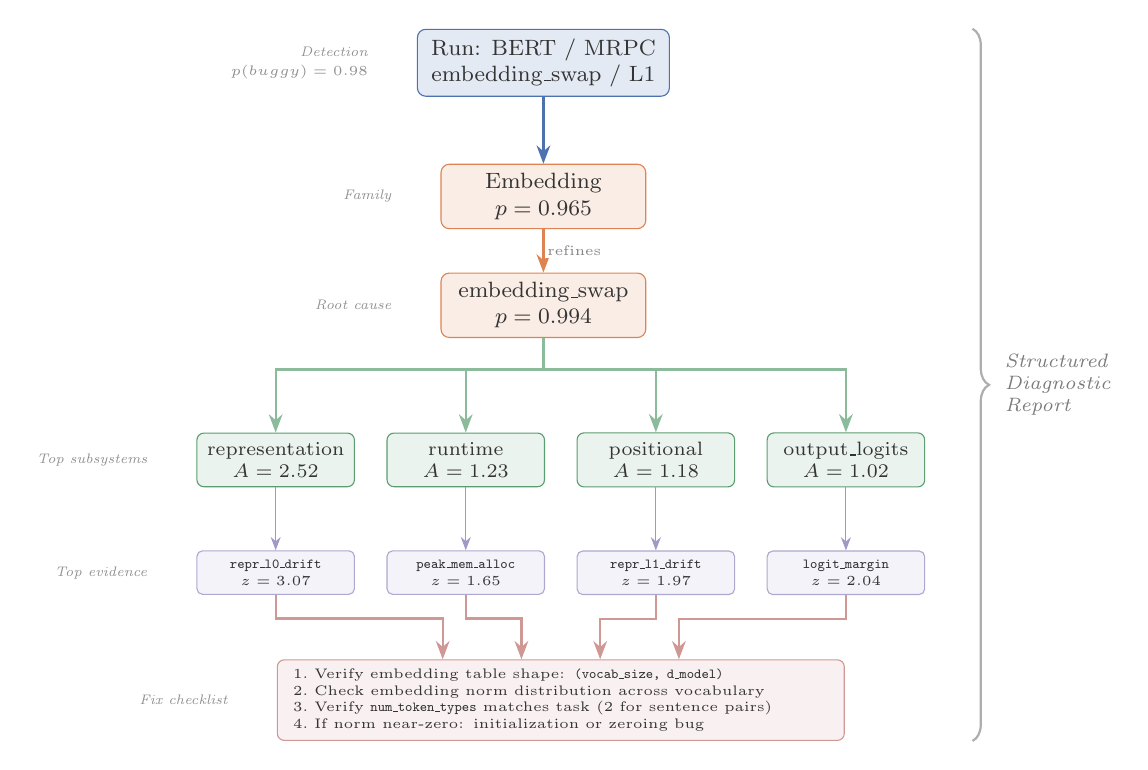
\begin{tikzpicture}[
  >=Stealth,
  every node/.style={font=\rmfamily\small, text=darkC},
  runbox/.style={draw=encC, fill=encC!15, rounded corners=3pt,
                 minimum width=3.2cm, minimum height=0.7cm,
                 font=\rmfamily\footnotesize, align=center},
  hypbox/.style={draw=hypC, fill=hypC!15, rounded corners=3pt,
                 minimum width=2.6cm, minimum height=0.6cm,
                 font=\rmfamily\footnotesize, align=center},
  subbox/.style={draw=subsC, fill=subsC!12, rounded corners=2.5pt,
                 minimum width=2.0cm, minimum height=0.55cm,
                 font=\rmfamily\scriptsize, align=center},
  featbox/.style={draw=featC!60, fill=featC!8, rounded corners=2pt,
                  minimum width=2.0cm, minimum height=0.45cm,
                  font=\ttfamily\tiny, align=center},
  fixbox/.style={draw=fixC!60, fill=fixC!8, rounded corners=2.5pt,
                 minimum width=7.2cm, minimum height=0.8cm,
                 font=\rmfamily\tiny, align=left, text width=6.8cm},
  phase/.style={font=\rmfamily\tiny\itshape, text=darkC!55},
  edgelbl/.style={font=\rmfamily\tiny, text=darkC!60, fill=white,
                  inner sep=1pt},
]

% ── Run ──
\node[runbox] (run) {Run: BERT / MRPC\\embedding\_swap / L1};

% ── Phase label: Detection ──
\node[phase, left=0.5 of run, align=right] (det)
  {Detection\\[1pt]$p(\text{buggy})=0.98$};

% ── Fault family ──
\node[hypbox, below=0.85 of run] (fam) {Embedding\\$p=0.965$};
\node[phase, left=0.5 of fam] {Family};

% ── Root cause ──
\node[hypbox, below=0.55 of fam] (root) {embedding\_swap\\$p=0.994$};
\node[phase, left=0.5 of root] {Root cause};

% ── Subsystems ──
\node[subbox, below=1.2 of root, xshift=-3.4cm] (s1) {representation\\$A=2.52$};
\node[subbox, right=0.4 of s1] (s2) {runtime\\$A=1.23$};
\node[subbox, right=0.4 of s2] (s3) {positional\\$A=1.18$};
\node[subbox, right=0.4 of s3] (s4) {output\_logits\\$A=1.02$};

\node[phase, left=0.5 of s1] {Top subsystems};

% ── Evidence features ──
\node[featbox, below=0.8 of s1] (f1) {repr\_l0\_drift\\$z=3.07$};
\node[featbox, below=0.8 of s2] (f2) {peak\_mem\_alloc\\$z=1.65$};
\node[featbox, below=0.8 of s3] (f3) {repr\_l1\_drift\\$z=1.97$};
\node[featbox, below=0.8 of s4] (f4) {logit\_margin\\$z=2.04$};

\node[phase, left=0.5 of f1] {Top evidence};

% ── Fix checklist ──
\node[fixbox, below=1.1 of $(f2)!0.5!(f3)$] (fix) {%
  1.~Verify embedding table shape: \texttt{(vocab\_size, d\_model)}\\
  2.~Check embedding norm distribution across vocabulary\\
  3.~Verify \texttt{num\_token\_types} matches task (2 for sentence pairs)\\
  4.~If norm near-zero: initialization or zeroing bug};

\node[phase, left=0.5 of fix] {Fix checklist};

% ── Edges: run -> family -> root ──
\draw[->, thick, encC] (run) -- (fam);
\draw[->, thick, hypC] (fam) -- node[edgelbl, right]{refines} (root);

% ── Root -> subsystems (fan out) ──
\draw[->, thick, subsC!70] (root.south) -- ++(0,-0.4) -| (s1.north);
\draw[->, thick, subsC!70] (root.south) -- ++(0,-0.4) -| (s2.north);
\draw[->, thick, subsC!70] (root.south) -- ++(0,-0.4) -| (s3.north);
\draw[->, thick, subsC!70] (root.south) -- ++(0,-0.4) -| (s4.north);

% ── Subsystems -> features ──
\draw[->, featC!70] (s1) -- (f1);
\draw[->, featC!70] (s2) -- (f2);
\draw[->, featC!70] (s3) -- (f3);
\draw[->, featC!70] (s4) -- (f4);

% ── Features -> fix (all four converge) ──
\draw[->, thick, fixC!60] (f1.south) -- ++(0,-0.3) -| ([xshift=-1.5cm]fix.north);
\draw[->, thick, fixC!60] (f2.south) -- ++(0,-0.3) -| ([xshift=-0.5cm]fix.north);
\draw[->, thick, fixC!60] (f3.south) -- ++(0,-0.3) -| ([xshift=0.5cm]fix.north);
\draw[->, thick, fixC!60] (f4.south) -- ++(0,-0.3) -| ([xshift=1.5cm]fix.north);

% ── Brace: Structured Diagnostic Report (opening to the LEFT, toward the diagram) ──
\draw[decorate, decoration={brace, amplitude=6pt},
      thick, darkC!40]
  ([xshift=0.6cm]s4.north east |- run.north) --
  ([xshift=0.6cm]s4.south east |- fix.south)
  node[midway, right=8pt, font=\rmfamily\scriptsize\itshape,
       text=darkC!65, align=left] {Structured\\Diagnostic\\Report};

\end{tikzpicture}
\end{document}
